\documentclass[leqno, 12pt]{article}
\usepackage{tikz}
\usetikzlibrary{positioning}
\usetikzlibrary {arrows.meta}
\usetikzlibrary{bending}
\usepackage[a4paper, portrait, margin=1cm]{geometry}
\pagestyle{empty}

\def\jumpheight{10}
\def\qgap{\rule[-1pt]{1.0em}{.25pt}}

\def \HeadingQuestions {\section*{\Large Name: \underline{\hspace{8cm}} \hfill Date: \underline{\hspace{3cm}}} \vspace{-3mm}
{Number lines: Questions} \vspace{1pt}\hrule}

\begin{document}
    \HeadingQuestions
    \vspace{-1mm}
    \begin{equation}
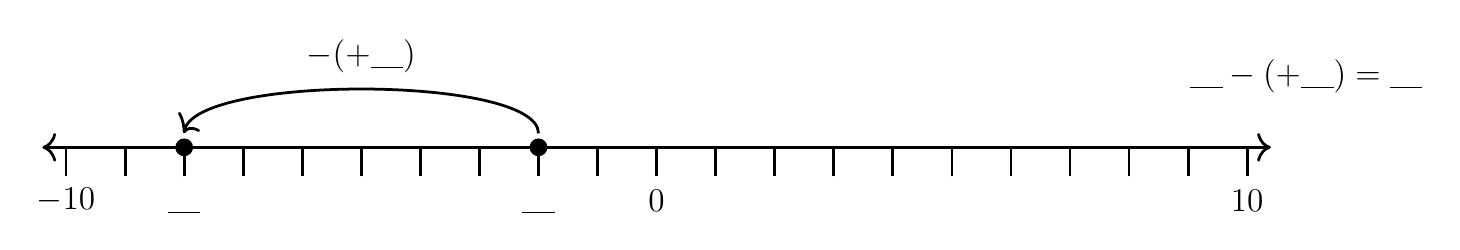
\begin{tikzpicture}[scale=0.75, baseline={([yshift=-1pt]current bounding box.north)}]
    % axis, arrow style to-to
    \draw[{To[scale=1.3]}-{To[scale=1.3]}, line width=1pt] (-10.4, 0) -- (10.4, 0);  
    % tick marks
    \foreach \x in {-10,-9,...,10}
        \draw[shift={(\x,0)},color=black, line width=1pt] (0pt,-14pt) -- (0pt,0pt);
    % numbers along each axis
    \foreach \x in {-10,0,10}
        \draw[shift={(\x,-0.8)},color=black] node[font=\large,text height=12pt] {$\x$};
    \draw[shift={(-2,-0.8)},color=black] node[font=\large,text height=12pt] {$\qgap$};
    \draw[shift={(-8,-0.8)},color=black] node[font=\large,text height=12pt] {$\qgap$};
    % dots
    \filldraw[black] (-2,0) circle (4pt) node[above,yshift=-2pt] (a) {};
    \filldraw[black] (-8,0) circle (4pt) node[above,yshift=-2pt] (b) {}; 
    % arrow
    \draw[-{To[scale=1.3, bend]},line width=1pt, color=black] (a.north)  .. controls  +(north:\jumpheight mm) and +(north:\jumpheight mm) .. node[above=2pt,font=\large,text height=10pt] {$-(+\qgap)$} (b.north); % for addition
    % equation at right end
    \node [font=\large, minimum width=30mm] at (11.0,1.2) {$\qgap - (+\qgap) = \qgap$};
\end{tikzpicture}
\end{equation}
\vspace{-2pt}\begin{equation}
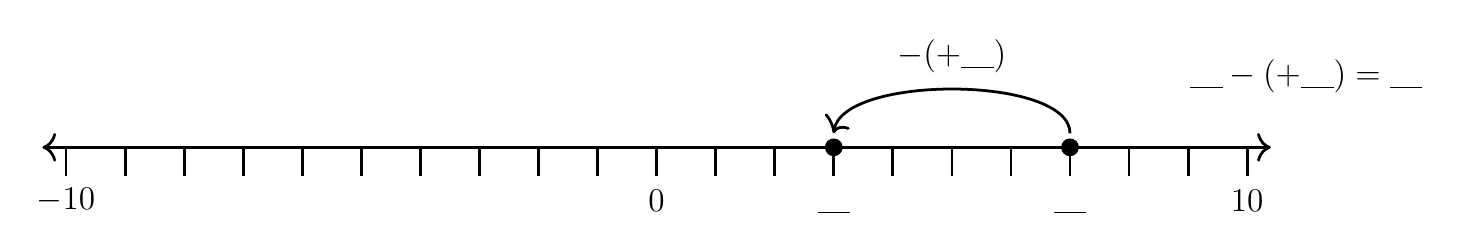
\begin{tikzpicture}[scale=0.75, baseline={([yshift=-1pt]current bounding box.north)}]
    % axis, arrow style to-to
    \draw[{To[scale=1.3]}-{To[scale=1.3]}, line width=1pt] (-10.4, 0) -- (10.4, 0);  
    % tick marks
    \foreach \x in {-10,-9,...,10}
        \draw[shift={(\x,0)},color=black, line width=1pt] (0pt,-14pt) -- (0pt,0pt);
    % numbers along each axis
    \foreach \x in {-10,0,10}
        \draw[shift={(\x,-0.8)},color=black] node[font=\large,text height=12pt] {$\x$};
    \draw[shift={(7,-0.8)},color=black] node[font=\large,text height=12pt] {$\qgap$};
    \draw[shift={(3,-0.8)},color=black] node[font=\large,text height=12pt] {$\qgap$};
    % dots
    \filldraw[black] (7,0) circle (4pt) node[above,yshift=-2pt] (a) {};
    \filldraw[black] (3,0) circle (4pt) node[above,yshift=-2pt] (b) {}; 
    % arrow
    \draw[-{To[scale=1.3, bend]},line width=1pt, color=black] (a.north)  .. controls  +(north:\jumpheight mm) and +(north:\jumpheight mm) .. node[above=2pt,font=\large,text height=10pt] {$-(+\qgap)$} (b.north); % for addition
    % equation at right end
    \node [font=\large, minimum width=30mm] at (11.0,1.2) {$\qgap - (+\qgap) = \qgap$};
\end{tikzpicture}
\end{equation}
\vspace{-2pt}\begin{equation}
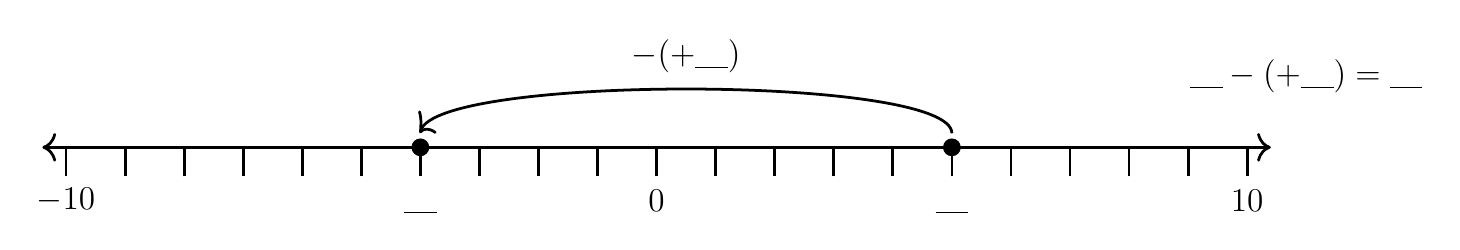
\begin{tikzpicture}[scale=0.75, baseline={([yshift=-1pt]current bounding box.north)}]
    % axis, arrow style to-to
    \draw[{To[scale=1.3]}-{To[scale=1.3]}, line width=1pt] (-10.4, 0) -- (10.4, 0);  
    % tick marks
    \foreach \x in {-10,-9,...,10}
        \draw[shift={(\x,0)},color=black, line width=1pt] (0pt,-14pt) -- (0pt,0pt);
    % numbers along each axis
    \foreach \x in {-10,0,10}
        \draw[shift={(\x,-0.8)},color=black] node[font=\large,text height=12pt] {$\x$};
    \draw[shift={(5,-0.8)},color=black] node[font=\large,text height=12pt] {$\qgap$};
    \draw[shift={(-4,-0.8)},color=black] node[font=\large,text height=12pt] {$\qgap$};
    % dots
    \filldraw[black] (5,0) circle (4pt) node[above,yshift=-2pt] (a) {};
    \filldraw[black] (-4,0) circle (4pt) node[above,yshift=-2pt] (b) {}; 
    % arrow
    \draw[-{To[scale=1.3, bend]},line width=1pt, color=black] (a.north)  .. controls  +(north:\jumpheight mm) and +(north:\jumpheight mm) .. node[above=2pt,font=\large,text height=10pt] {$-(+\qgap)$} (b.north); % for addition
    % equation at right end
    \node [font=\large, minimum width=30mm] at (11.0,1.2) {$\qgap - (+\qgap) = \qgap$};
\end{tikzpicture}
\end{equation}
\vspace{-2pt}\begin{equation}
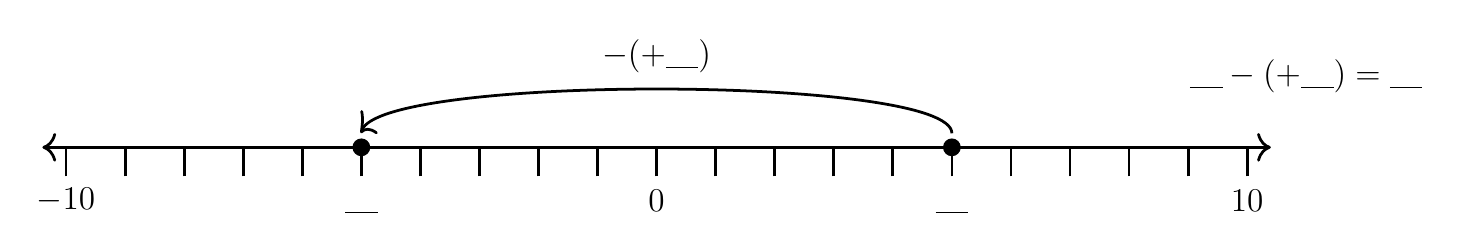
\begin{tikzpicture}[scale=0.75, baseline={([yshift=-1pt]current bounding box.north)}]
    % axis, arrow style to-to
    \draw[{To[scale=1.3]}-{To[scale=1.3]}, line width=1pt] (-10.4, 0) -- (10.4, 0);  
    % tick marks
    \foreach \x in {-10,-9,...,10}
        \draw[shift={(\x,0)},color=black, line width=1pt] (0pt,-14pt) -- (0pt,0pt);
    % numbers along each axis
    \foreach \x in {-10,0,10}
        \draw[shift={(\x,-0.8)},color=black] node[font=\large,text height=12pt] {$\x$};
    \draw[shift={(5,-0.8)},color=black] node[font=\large,text height=12pt] {$\qgap$};
    \draw[shift={(-5,-0.8)},color=black] node[font=\large,text height=12pt] {$\qgap$};
    % dots
    \filldraw[black] (5,0) circle (4pt) node[above,yshift=-2pt] (a) {};
    \filldraw[black] (-5,0) circle (4pt) node[above,yshift=-2pt] (b) {}; 
    % arrow
    \draw[-{To[scale=1.3, bend]},line width=1pt, color=black] (a.north)  .. controls  +(north:\jumpheight mm) and +(north:\jumpheight mm) .. node[above=2pt,font=\large,text height=10pt] {$-(+\qgap)$} (b.north); % for addition
    % equation at right end
    \node [font=\large, minimum width=30mm] at (11.0,1.2) {$\qgap - (+\qgap) = \qgap$};
\end{tikzpicture}
\end{equation}
\vspace{-2pt}\begin{equation}
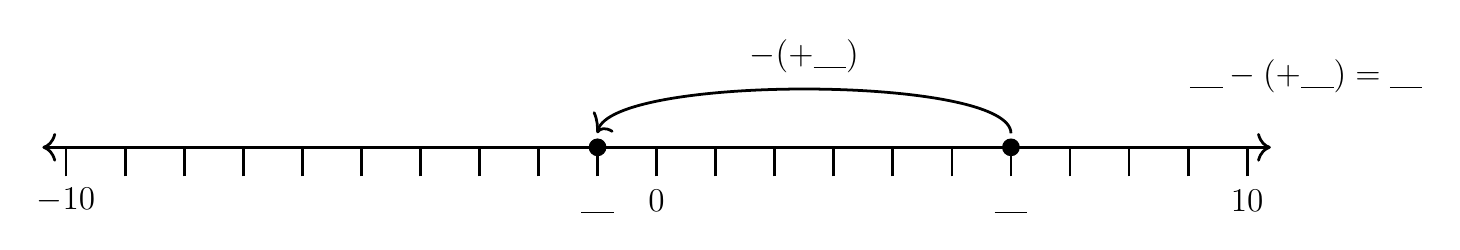
\begin{tikzpicture}[scale=0.75, baseline={([yshift=-1pt]current bounding box.north)}]
    % axis, arrow style to-to
    \draw[{To[scale=1.3]}-{To[scale=1.3]}, line width=1pt] (-10.4, 0) -- (10.4, 0);  
    % tick marks
    \foreach \x in {-10,-9,...,10}
        \draw[shift={(\x,0)},color=black, line width=1pt] (0pt,-14pt) -- (0pt,0pt);
    % numbers along each axis
    \foreach \x in {-10,0,10}
        \draw[shift={(\x,-0.8)},color=black] node[font=\large,text height=12pt] {$\x$};
    \draw[shift={(6,-0.8)},color=black] node[font=\large,text height=12pt] {$\qgap$};
    \draw[shift={(-1,-0.8)},color=black] node[font=\large,text height=12pt] {$\qgap$};
    % dots
    \filldraw[black] (6,0) circle (4pt) node[above,yshift=-2pt] (a) {};
    \filldraw[black] (-1,0) circle (4pt) node[above,yshift=-2pt] (b) {}; 
    % arrow
    \draw[-{To[scale=1.3, bend]},line width=1pt, color=black] (a.north)  .. controls  +(north:\jumpheight mm) and +(north:\jumpheight mm) .. node[above=2pt,font=\large,text height=10pt] {$-(+\qgap)$} (b.north); % for addition
    % equation at right end
    \node [font=\large, minimum width=30mm] at (11.0,1.2) {$\qgap - (+\qgap) = \qgap$};
\end{tikzpicture}
\end{equation}
\vspace{-2pt}\begin{equation}
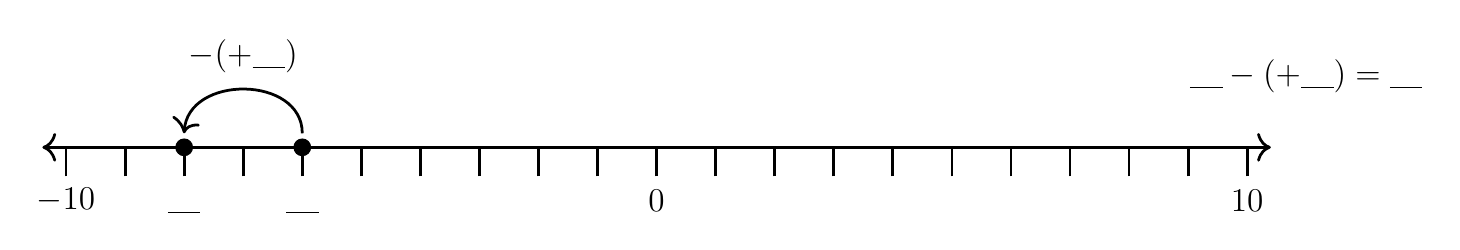
\begin{tikzpicture}[scale=0.75, baseline={([yshift=-1pt]current bounding box.north)}]
    % axis, arrow style to-to
    \draw[{To[scale=1.3]}-{To[scale=1.3]}, line width=1pt] (-10.4, 0) -- (10.4, 0);  
    % tick marks
    \foreach \x in {-10,-9,...,10}
        \draw[shift={(\x,0)},color=black, line width=1pt] (0pt,-14pt) -- (0pt,0pt);
    % numbers along each axis
    \foreach \x in {-10,0,10}
        \draw[shift={(\x,-0.8)},color=black] node[font=\large,text height=12pt] {$\x$};
    \draw[shift={(-6,-0.8)},color=black] node[font=\large,text height=12pt] {$\qgap$};
    \draw[shift={(-8,-0.8)},color=black] node[font=\large,text height=12pt] {$\qgap$};
    % dots
    \filldraw[black] (-6,0) circle (4pt) node[above,yshift=-2pt] (a) {};
    \filldraw[black] (-8,0) circle (4pt) node[above,yshift=-2pt] (b) {}; 
    % arrow
    \draw[-{To[scale=1.3, bend]},line width=1pt, color=black] (a.north)  .. controls  +(north:\jumpheight mm) and +(north:\jumpheight mm) .. node[above=2pt,font=\large,text height=10pt] {$-(+\qgap)$} (b.north); % for addition
    % equation at right end
    \node [font=\large, minimum width=30mm] at (11.0,1.2) {$\qgap - (+\qgap) = \qgap$};
\end{tikzpicture}
\end{equation}
\vspace{-2pt}\begin{equation}
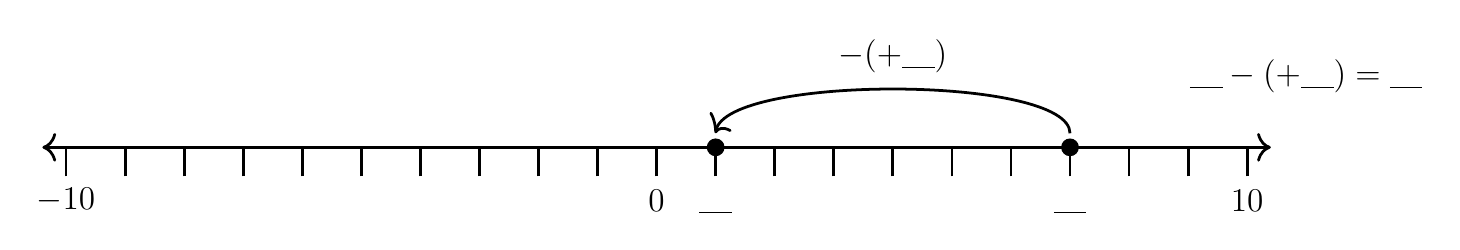
\begin{tikzpicture}[scale=0.75, baseline={([yshift=-1pt]current bounding box.north)}]
    % axis, arrow style to-to
    \draw[{To[scale=1.3]}-{To[scale=1.3]}, line width=1pt] (-10.4, 0) -- (10.4, 0);  
    % tick marks
    \foreach \x in {-10,-9,...,10}
        \draw[shift={(\x,0)},color=black, line width=1pt] (0pt,-14pt) -- (0pt,0pt);
    % numbers along each axis
    \foreach \x in {-10,0,10}
        \draw[shift={(\x,-0.8)},color=black] node[font=\large,text height=12pt] {$\x$};
    \draw[shift={(7,-0.8)},color=black] node[font=\large,text height=12pt] {$\qgap$};
    \draw[shift={(1,-0.8)},color=black] node[font=\large,text height=12pt] {$\qgap$};
    % dots
    \filldraw[black] (7,0) circle (4pt) node[above,yshift=-2pt] (a) {};
    \filldraw[black] (1,0) circle (4pt) node[above,yshift=-2pt] (b) {}; 
    % arrow
    \draw[-{To[scale=1.3, bend]},line width=1pt, color=black] (a.north)  .. controls  +(north:\jumpheight mm) and +(north:\jumpheight mm) .. node[above=2pt,font=\large,text height=10pt] {$-(+\qgap)$} (b.north); % for addition
    % equation at right end
    \node [font=\large, minimum width=30mm] at (11.0,1.2) {$\qgap - (+\qgap) = \qgap$};
\end{tikzpicture}
\end{equation}
\vspace{-2pt}\begin{equation}
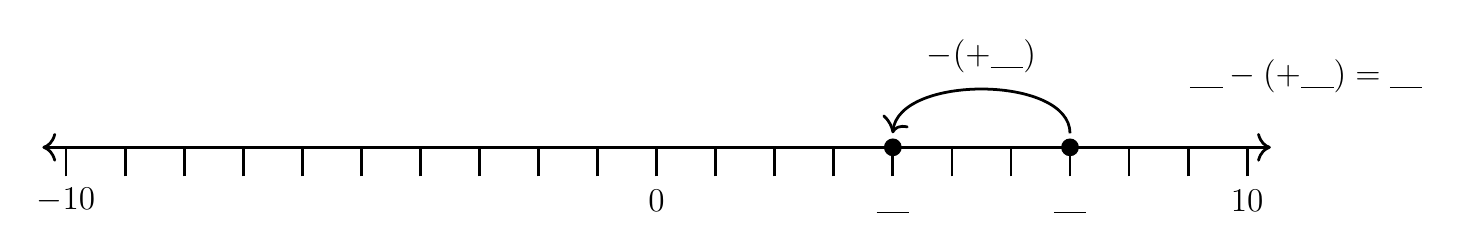
\begin{tikzpicture}[scale=0.75, baseline={([yshift=-1pt]current bounding box.north)}]
    % axis, arrow style to-to
    \draw[{To[scale=1.3]}-{To[scale=1.3]}, line width=1pt] (-10.4, 0) -- (10.4, 0);  
    % tick marks
    \foreach \x in {-10,-9,...,10}
        \draw[shift={(\x,0)},color=black, line width=1pt] (0pt,-14pt) -- (0pt,0pt);
    % numbers along each axis
    \foreach \x in {-10,0,10}
        \draw[shift={(\x,-0.8)},color=black] node[font=\large,text height=12pt] {$\x$};
    \draw[shift={(7,-0.8)},color=black] node[font=\large,text height=12pt] {$\qgap$};
    \draw[shift={(4,-0.8)},color=black] node[font=\large,text height=12pt] {$\qgap$};
    % dots
    \filldraw[black] (7,0) circle (4pt) node[above,yshift=-2pt] (a) {};
    \filldraw[black] (4,0) circle (4pt) node[above,yshift=-2pt] (b) {}; 
    % arrow
    \draw[-{To[scale=1.3, bend]},line width=1pt, color=black] (a.north)  .. controls  +(north:\jumpheight mm) and +(north:\jumpheight mm) .. node[above=2pt,font=\large,text height=10pt] {$-(+\qgap)$} (b.north); % for addition
    % equation at right end
    \node [font=\large, minimum width=30mm] at (11.0,1.2) {$\qgap - (+\qgap) = \qgap$};
\end{tikzpicture}
\end{equation}
\vspace{-2pt}
\end{document}
